%\documentclass[10pt, twocolumn]{article}
\documentclass[twocolumn,showpacs,preprintnumbers,amsmath,amssymb,prd]{revtex4}
%\documentclass[11 pt,preprint,preprintnumbers,amsmath,amssymb, prd]{revtex4}

% Preamble adapted from Surjeet Rajendran

\usepackage{latexsym}
\usepackage{amssymb}
\usepackage{epsfig,amsmath,graphics}
\usepackage{epstopdf}
\usepackage{verbatim}
\usepackage{wasysym}
\usepackage{hyperref}
\usepackage{feynmp-auto} % feynman diagrams
%\usepackage{subfig}
\usepackage[utf8]{inputenc}
\usepackage{xpatch}
\usepackage{xcolor}
\hypersetup{
    colorlinks,
    linkcolor={red!80!black},
    citecolor={green!60!black},
    urlcolor={blue!60!black}
}
\usepackage{appendix}

\newcommand{\Ez}{\mathcal{E}_0}
\newcommand{\Eboom}{\mathcal{E}_\text{boom}}

\newcommand{\OO}{\mathcal{O}}
\newcommand{\LL}{\mathcal{L}}
\newcommand{\HH}{\mathcal{H}}

\newcommand{\TeV}{\text{TeV}}
\newcommand{\GeV}{\text{GeV}}
\newcommand{\MeV}{\text{MeV}}
\newcommand{\keV}{\text{keV}}
\newcommand{\rad}{\text{rad}}
\newcommand{\cm}{\text{cm}}
\newcommand{\angstrom}{\buildrel _{\circ} \over {\mathrm{A}}}
\newcommand{\pslash}{p\hspace{-0.070in}/\,}
\newcommand{\Mpl}{M_{\text{pl}}}
\newcommand{\ket}[1]{\ensuremath{\left|#1\right>}}
\newcommand{\bra}[1]{\ensuremath{\left<#1\right|}}
\newcommand{\braket}[2]{\ensuremath{\left<#1|#2\right>}}
%Large Parentheses
\def\r{\right)}
\def\l{\left(}

\begin{document}

\title{White Dwarfs as Dark Matter Detectors}

\author{Ryan Janish}
\affiliation{Berkeley Center for Theoretical Physics, Department of Physics,
University of California, Berkeley, CA 94720, USA}

\author{Vijay Narayan}
\affiliation{Berkeley Center for Theoretical Physics, Department of Physics,
University of California, Berkeley, CA 94720, USA}

\author{Surjeet Rajendran}
\affiliation{Berkeley Center for Theoretical Physics, Department of Physics,
University of California, Berkeley, CA 94720, USA}

\author{Paul Riggins}
\affiliation{Berkeley Center for Theoretical Physics, Department of Physics,
University of California, Berkeley, CA 94720, USA}

\begin{abstract}

White dwarfs can serve as detectors for ultra-heavy dark matter states which interact to trigger type Ia supernovae.
This was originally proposed in \cite{Graham:2015apa} and used to place bounds on primordial black holes.
In this paper, we extend the reach of white dwarf detectors to dark matter candidates with non-gravitational couplings that release energy in the form of standard model particles.
This is used to constrain dark matter models which can ignite white dwarfs through annihilations, decays, or transits.
As a concrete example, we are able to constrain supersymmetric Q-ball dark matter in a vast region of parameter space fundamentally inaccessible to terrestrial-based experiments.


\end{abstract}
\maketitle
%\tableofcontents
%\newpage

\section{Introduction}
\label{sec:Introduction}

The detection of ultra-heavy dark matter (DM) is an open problem which will likely require a confluence of astrophysical probes.
For instance, DM masses above $\sim 10^{22} ~\GeV$ will register fewer than a single event per year in a typical terrestrial detector of size $\sim (100 ~\text{m})^2$.
Furthermore, the lack of conclusive signatures on a variety of experimental fronts has led many to consider DM candidates far above the weak scale and their potential signatures \textcolor{blue}{add few citations}.
One possibility proposed by \cite{Graham:2015apa} is that DM can trigger supernovae (SN) in sub-Chandrasekhar white dwarf (WD) stars by inducing runaway fusion.
As such, white dwarfs can serve as detectors for ultra-heavy DM states.

White dwarfs are particularly suited to this task as they are more susceptible to runaway fusion than are main-sequence stars.
Runaway fusion requires that two criteria be met: a region within the star must be hot enough to support exothermic fusion reactions, and the rate at which energy is released must dominate any cooling mechanisms that drain energy from the fusing region.
Since the pressure of a WD is set by electron degeneracy and is thus independent of temperature, thermal expansion is suppressed as a potential cooling mechanism.
Therefore WD cooling relies on thermal diffusion, which becomes less important over longer length scales, and can be overcome by sufficiently heating a large enough region of the WD.

The necessary trigger for runaway fusion was initially computed in \cite{Woosley} and recently implemented in \cite{Graham:2015apa} to place bounds on primordial black holes. 
In addition, the authors of \cite{Graham:2015apa} identify several other heating mechanisms involving DM which may be constrained in a similar manner.
In this paper, we extend the reach of WD detectors to DM candidates with non-gravitational couplings which release energy in the form of high-energy standard model (SM) particles.
DM models with interactions of this sort include Q-balls found in supersymmetric extensions of the SM and dark nuclei with higher-dimension couplings to the SM \cite{Hardy:2014mqa}.
An essential ingredient in this analysis is an understanding of how individual SM particles deposit energy in a WD medium through strong and electromagnetic interactions. 
In this regard, the WD may be thought of as a detector with hadronic and electromagnetic ``calorimeter'' components.
This is used to constrain DM models which can ignite WDs via DM-DM collisions, DM decays, or transits with a DM-SM scattering interaction. 
The proposed bounds will come from either observing specific, long-lived white dwarfs or comparing the measured type Ia SN rate with the expected rate due to DM events.
As a concrete example, we are able to constrain Q-ball DM in regions of parameter space fundamentally inaccessible to terrestrial experiments.
However, it is important to note that any such DM constraints are by nature complimentary to terrestrial ones - it is more massive DM that is likely to trigger SN, and also more massive DM that has sufficiently low flux on Earth.
What allows the WD detector to be effective in this regime is its enhanced surface area $\sim (10^4 ~\text{km})^2$, exceptionally long lifetime $\sim \text{Gyr}$, and astronomical abundance in the galaxy. 

We begin in Section~\ref{sec:Review} by reviewing the mechanism of runaway fusion in a WD. 
The ability for DM to trigger SN through non-gravitational interactions is ultimately based on the heating properties of ordinary SM particles, which is summarized in Section~\ref{sec:SMHeating} for different species and energies.
In Section~\ref{sec:DMexplode} we derive conditions on the properties of DM necessary to ignite white dwarfs, and in Section~\ref{sec:Constraints} we constrain DM models with interactions parameterized by a simple, schematic form.  
We examine the specific case of Q-balls in Section~\ref{sec:QBalls}, and conclude in Section~\ref{sec:Discussion}.

\section{White Dwarf Runaway Fusion}
\label{sec:Review}

Any process which deposits energy in a WD will eventually heat a localized region within the star. 
Since we are interested in nuclear fusion, let $L_0$ be the length scale of the local peak in ion temperature $T_0$ and $\Ez \sim n_\text{ion} T_0 L_0^3$ be the excess thermal energy it contains, where $n_\text{ion}$ is the number density of ions. 
Note that the size and thermal properties of any heated region will evolve in time, so we take $L_0$ and $\Ez$ to characterize this peak as it initially forms, i.e.\ immediately after a temperature profile for ions has been established.
Thus for a given heating event, $L_0$ is a measure of the efficiency with which the energy deposit is transferred to ions in the stellar medium.
This may vary significantly with the form of the energy deposit and with WD density.
For example, suppose that kinetic energy is transferred directly to a single ion through a short-range elastic scatter.
This ion would thermalize with neighboring ions, resulting in a heating length $L_0$ of order the ion mean free path.
In the other extreme, suppose that a process produces electrons in the WD at energies just above the Fermi energy.
These electrons have Pauli-suppressed interactions and will travel a long distance before their energy is scattered and thermalized among ions, resulting in a much larger $L_0$.

The fate of a locally heated region in a WD is either a nonviolent diffusion of the energy deposit across the star, or a runaway fusion chain-reaction that will destroy the star.
The precise outcome is governed by two parameters: the fusion temperature $T_f$ and trigger size $\lambda_T$.
The fusion temperature $T_f$ is the threshold for the onset of fusion and is given by the energy required for ions to overcome their mutual Coulomb barrier.
In carbon-oxygen WDs, this is a constant $T_f \sim \MeV$ \textcolor{blue}{SR cite}.
However, while any region with $T_0 > T_f$ will initially support fusion, this condition is not sufficient for triggering a runaway process.
Sustained heating through nuclear fusion can only be maintained if the timescale for cooling is consistently longer than the timescale for heating. 
Cooling in a WD is dominated by diffusion and the characteristic diffusion time for a heated region increases with its size while the rate of fusion is independent of size. 
Therefore, there will always be a critical size of a heated region (at fixed temperature) above which fusion is maintained as the dominant thermal process.
For a region at the threshold of nuclear fusion $T_f$, this condition defines the trigger size $\lambda_T$.
The value of $\lambda_T$ is highly dependent on stellar density, and is set by either the thermal diffusivity of photons or degenerate electrons.
It has been calculated numerically in \cite{Woosley} and analytically scaled for varying WD masses in \cite{Graham:2015apa}.
As in \cite{Graham:2015apa}, we restrict our attention to carbon-oxygen WDs in the upper mass range $\sim 0.7 - 1.4 ~M_{\odot}$ which correspond to a central number density of ions $n_\text{ion} \sim 10^{29} - 10^{32} ~\cm^{-3}$.
Over this range, the trigger size is approximately $\lambda_T \sim 10^{-5} - 10^{-2} ~\text{cm}$.

In summary, a local temperature peak $T_f$ in a WD will either always be dominated by diffusive cooling if $L_0 < \lambda_T$ or sustained fusion if $L_0 > \lambda_T$.  
However, there is an additional possibility if $T_0 > T_f$ that the thermal evolution is initially dominated by diffusion but at a later time results in runaway fusion. 
We can assess this outcome by assuming the region with $T_0 > T_f$ begins to diffuse and cool until its temperature reaches $\sim T_f$.
If the size of the region at this point is larger than $\lambda_T$, a runaway will occur.  
For a heated region of initial size $L_0$ and total energy deposit $\Ez$, the condition to trigger a type Ia SN via runaway fusion is
\begin{equation}
\label{eq:boom}
  \Ez \gtrsim n_\text{ion} T_f \text{max}\{L_0, \lambda_T\}^3.
\end{equation}
This implies the explosion condition used in \cite{Graham:2015apa}, but also provides a less stringent criteria applicable to regions of temperature greater than $T_f$ and size less than $\lambda_T$ which was not needed in that work.  
Thus there is an absolute minimum energy required to ignite a WD
\begin{equation}
\label{eq:Eboom}
\mathcal{E}_{\text{boom}} \sim n_\text{ion} T_f \lambda_T^3 \sim 10^{15} - 10^{22} ~\GeV,
\end{equation}
where $\mathcal{E}_{\text{boom}} $ varies with trigger size $\lambda_T$ over the range of WD densities.
This is plotted in Figure \ref{fig:Eboom}.
Note that the threshold \eqref{eq:Eboom} is only sufficient if the deposited energy thermalizes within a region of size $L_0 < \lambda_T$.
The threshold energy for explosion is parametrically larger if energy is deposited on a larger length scale $L_0 > \lambda_T$.
As a result, understanding the heating length $L_0$ of a process is critical to determining whether or not it is capable of destroying a WD. 
\begin{figure}
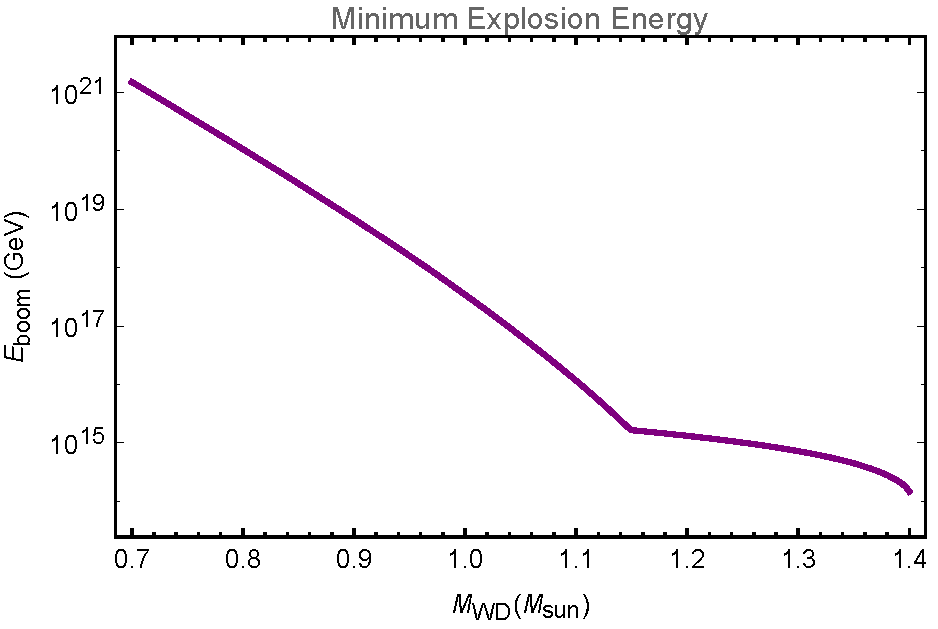
\includegraphics[scale=.45]{Eboom.pdf}
\caption{Minimum energy $\Eboom$ required to trigger SN as a function of WD mass, based on numerical results for $\lambda_T$ \cite{Woosley}.}
\label{fig:Eboom}
\end{figure}

\section{Dark Matter and Non-Gravitational Heating of White Dwarfs}
\label{sec:SMHeating}

Having reviewed the requirements for runaway fusion in a WD, we turn to the question of triggering these events with DM. 
This amounts to determining the heating length $L_0$ and energy deposit $\Ez$ due to a given DM encounter with a WD - if condition \eqref{eq:boom} is satisfied, then the encounter is explosive.
Of course, the parameters $L_0$ and $\Ez$ necessarily depend on the nature of the DM and must be explicitly calculated for a given DM model. 
This was done in \cite{Graham:2015apa} in the case of primordial black holes, which deposit energy through dynamical friction while transiting the star.
However, non-gravitational interactions also have the potential to trigger SN. 
In particular, any DM candidate which couples to the SM will generically be able to release SM secondaries which then thermalize with stellar constituents. 
For these types of processes, the unknown DM physics serves only to determine the initial distribution in space, energy, and species of the SM particles produced in the star, while the actual heating proceeds entirely though known SM interactions. 
It is therefore necessary to understand how energy is transferred from SM particles to the stellar medium in order to assess the explosiveness of these encounters.
If the energy of SM secondaries is sourced from the energy of the non-relativistic DM, then the DM mass must be greater than \eqref{eq:Eboom}.
Thus we are sensitive to ultra-heavy $>10^{15} ~\GeV$ DM particles, most likely composite states, which interact in the WD to produce either a few ultra-high energy particles or many lower energy particles.
As the lightest SM particles will be most typically produced, we focus on the release of light hadrons, electrons, and photons and neutrinos. 

The remainder of this Section is dedicated to computing the heating properties of these SM species in a manner that is independent of the precise DM encounter. 
Consider a schematic energy deposition in which $N$ particles of a single SM species and uniform energy $\epsilon$ are released isotropically in the stellar interior.
As we are only concerned with triggering runaway fusion, it is sufficient to take $\epsilon \gg T_f \sim \text{MeV}$. 
In order to assess the heating length of this deposition, it is necessary to calculate the distance a particle travels before giving up an $\OO(1)$ fraction of its energy to nuclei.
We summarize here as needed the dominant source of energy loss for each species while a more detailed treatment of particle interactions in a WD is reserved for Appendix \ref{sec:Appendix}.
For every possible interaction of a given species described by a stopping power $(dE/dx)$, we define a length scale $\lambda \sim (dE/dX)^{-1} E$ as the range over which that species deposits its energy to either stellar constituents or to additional secondaries. 
The physical parameter which determines the explosiveness of such a schematic deposition is the resulting width $R$ of the initial ion temperature peak that forms. 
As a benchmark, the value of $\Delta$ for any species should be compared to the trigger size $\lambda_T$ in order to gauge the efficiency with which it deposits energy. 
It is important to note that any net displacement of this ion temperature profile from the point of origin of released SM particles is irrelevant for the sake of triggering runaway fusion. 
If $N \gg 1$ this displacement is negligible but for $N \sim 1$ it could be much larger than $\Delta$. 
We take care to distinguish the heating in this two scenarios when applicable.


\subsection{Heating Properties of Hadrons}

First we consider the energy loss of low-energy hadrons less than the nuclear binding energy $\epsilon \lesssim E_\text{nuc} \sim 10 ~\text{MeV}$. 
At these energies, protons and neutrons are stopped predominantly through elastic nuclear scatters, characterized by a typical mean free path
\begin{equation}
l_\text{h,el} \sim 1/n_\text{ion} \sigma_\text{h,el} \approx 10^{-7} ~\text{cm} 
\end{equation}
Thermalization of ions will occur after these nucleons have transferred $\OO(1)$ of their energy in the form of a random walk, which occurs after $\sim 10$ nuclear collisions. 
On the other hand, for charged pions the dominant stopping mechanism is to transfer energy to electrons in the stellar medium through Coulomb collisions.
In this case, the heating of ions depends on the distance over which electrons below $\sim 10~\MeV$ are able to scatter off ions. 
As shown in Figure \ref{fig:SOMETHING}, there are effectively no processes that efficiently transfer energy from electrons to ions at these energies. 
This is to be expected since these electrons can acquire a temperature at most just above the Fermi energy and disperse their energy over a large and therefore insignificant region. 

For hadrons of energy $\epsilon > 10 ~\text{MeV}$, the energy loss is dominated by nonelastic nuclear collisions in which an incoming hadron strongly interacts with a target nuclear constituent to produce several secondary hadrons.
The remaining nucleus is left in an excited state of energy $\sim 10 ~\text{MeV}$ with negligible center-of-mass recoil \textcolor{blue}{cite}, while the incident energy is transferred almost entirely to secondaries.
At sufficiently high energies, the result will be a roughly collinear hadronic shower. 
Shower constituents will tend to be pions and nucleons in roughly equal fractions, along with a few heavier states, i.e.\ deuterons, alpha particles, etc.\ \textcolor{blue}{citation}
The energy loss of a hadronic shower is set by the typical mean free path for nonelastic collisions with nuclei in the WD $l_\text{h,non} \sim 1/n_\text{ion} \sigma_\text{h,non}$. 
with the key length scale being $l_\text{h,non} \sim 1/n_\text{ion} \sigma_\text{h,non}$, the typical mean free path for nonelastic collisions with nuclei in the WD.
The shower terminates when constituents reach the critical energy $\sim 10 ~\text{MeV}$, so that the shower length $X_{\text{had}}$ is of order
\begin{align}
\label{eq:hadlength}
  X_{\text{had}} \sim l_\text{h,non} \log\l\frac{\epsilon}{E_\text{nuc}}\r
  \approx 10 ~l_\text{h,non}.
\end{align}
Therefore a high-energy nucleon or pion ultimately transfers its energy to many low-energy $\sim 10 ~\text{MeV}$ hadrons, displaced a distance $X_\text{had}$ from its starting point.
Note that while neutrons and $\pi^\pm$ are long-lived, neutral pions decay to photons with a mean lifetime $\sim 10^{-16} ~\text{s}$. 
For instance, a $10 ~\text{MeV}$ neutral pion has a decay length of order $\sim 10^{-6} ~\text{cm}$ while more relativistic $\pi^0$ can travel much further.
Hence, there will be electromagnetic contributions from $\pi^0$ decays during the progression of a hadronic shower for all but the most dense WDs. 
These will 
 

The energy loss of these shower products is determined as above - nucleons (and any heavier hadrons) will efficiently heat ions via elastic nuclear scatters while charged pions will instead heat electrons. 
As each nucleon and pion species carries roughly an $\OO(1)$ fraction of the initial energy, we may simple ignore the energy lost into electrons.
Thus $\OO(1)$ of the shower energy will thermalize with ions over a distance set by the mean free path for elastic scatters $ l_\text{h,el}$. 

We now state the results for hadrons released in the WD at arbitrary energies. The hadronic shower is mostly collinear, so a single high-energy hadron will produce an ion temperature profile of size $\Delta \approx\lambda_\text{nuc,el}$ that is displaced a distance $X_\text{had}$ from its starting point. 
If many low-energy hadrons are released and thermalize collectively, they will produce an ion profile centered on their origin with size $\Delta \approx X_\text{had} + \lambda_\text{nuc,el}$.
These two scales are
\begin{align}
  X_\text{had} \sim 10 ~l_\text{h,non}
  &\sim 10^{-6} ~\text{cm} \l\frac{10^{32}~\text{cm}^{-3}}{n_\text{ion}}\r \\ 
  \lambda_\text{nuc,el} \sim \sqrt{10} \times l_\text{h,el}  
  &\sim  10^{-7} ~\text{cm} \l\frac{10^{32}~\text{cm}^{-3}}{n_\text{ion}}\r
\end{align}
Here we have assumed characteristic values for the nuclear cross-sections $\sigma_\text{h,el} \approx 10~\sigma_\text{h,non} \approx 1~\text{barn}$ that are consistent with existing data. constant with incoming particle energy \textcolor{blue}{citation}.
Note that $X_\text{had}$ dominates in the many-particle case and a more compact heating is achieved with a single high-energy hadron. 
However, both of these scales are below the trigger size for the most massive WDs, and so either mechanism will result in ignition with the deposit of the minimal energy $\Eboom$. 



\subsection{Heating Properties of Electrons and Photons}

The stopping of electrons and photons in a WD are shown in Figures \ref{fig:SPelectron} and \ref{fig:SPphoton}, and we consider the heating properties of these species together as their interactions are highly coupled.  
However, stopping powers are more complicated than hadrons, in particular due to a sharp density dependence. 
Generally, they will both lose energy via radiative processes involving soft ion scatters (bremsstrahlung and electron-positron pair production), however at sufficiently high WD density these processes are highly suppressed due to efficient charge screening by degenerate electrons.  
This is manifest in a critical ion density $n_\text{EM} \sim 10^{31} ~\text{cm}^{-3}$, corresponding to a critical WD mass $M_\text{EM} \sim $ \textcolor{blue}{MASS}, above which radiative processes can be ignored. 
We will first consider the heating properties of electrons and photons for $M_\text{WD} \lesssim M_\text{EM}$, and then discuss the correction necessary for $M_\text{WD} \gtrsim M_\text{EM}$.
 
At low energies, $\epsilon \lesssim 10~\GeV$, both electrons and photons primarily lose energy via elastic scattering off WD electrons.
Thus the first stage of heating will be to establish a region of heated electron gas.
Once the electrons equilibrate, they will begin to further lose energy via the previously sub-dominant bremsstrahlung process - this increases the photon number density, which transfers energy back into electrons by Compton scatters, and will eventually lead to the thermalization of the electrons and photon. 
The establishment of this heated electron-photon gas will occur significantly before any energy is transfered to ions, as evidenced by the hierarchy between the electron-ion and photon-ion stopping powers and the election-photon stopping powers in Figure \ref{fig:SOMETHING}.
If the process originally released $N$ electrons or photons of energy $\epsilon \lesssim 10~\GeV$, then this electron-photon gas has a temperature of 
\begin{align}
  T_{e\gamma} \sim \frac{N \epsilon}{Z n_\text{ion} \lambda_{e\gamma}^3}
\end{align}
where $\lambda_{e\gamma}$ is the range of electrons due to bremsstrahlung and we assume that $N$ is sufficiency large so that $T_{e\gamma} \gtrsim 1~\MeV$.  

Note that if $T_{e\gamma} \lesssim 10~\MeV$, the only routes to transfer energy to ions are dramatically suppressed, as discussed in Section \ref{sec:SOMETHING}. 
In that case, ion heating is dispersed over an insignificantly large region. 
However, if $T_{e\gamma} \gtrsim 10~\MeV$, then photons in this gas will transfer their energy to ions via photonuclear scatters, which are nonelastic nuclear scatters as discussed in Section \ref{sec:SOMETHING} between a photon and a nucleus, mediated by a virtual quark pair.   
As $N$ is large and each photon carries a small fraction of the total deposited energy, the effect here is to launch many hadronic showers from the electron-photon gas which heat ions as discussed in Section \ref{sec:SOMETHING}.  
The total length of these photo-nuclear showers is given by $l_\gamma + X_\text{had}$, where $X_\text{had}$ is the hadronic shower length and $l_\gamma$ the mean free path for a photonuclear collision, which is related to the hadronic mean free path for nonelastic nuclear collisions by $\sim l_\text{h,non}/\alpha$.
The photonuclear piece dominates, and it also dominates the initial scale of the heated electrons and photons $\lambda_{e\gamma}$, so we find that a low-energy cloud of electrons or photons will eventually heat ions over a distance $\sim l_\gamma$.

For slightly larger energies, there is a narrow window $10~\GeV \lesssim \epsilon \lesssim 100~\GeV$ in which both electrons and photons are dominated by radiative processes.
In this regime we thus have an EM shower, which terminated at energies of $\sim 10~\GeV$ into a cloud of electrons and photons, which thermalize as described above.
This is a collinear shower covering about a decade in energy, so its principle effect is to amplify the number of energetic particles by a factor of $10$ and to disperse them over an EM shower length (note that since many particles are necessary involved here, this is a broadening of the heating peak and not a displacement).
If $N$ electrons or photons are released with energy $\epsilon$ and create EM showers, the shower products with thermalize an electron-photon gas of temperature  
\begin{align}
  T_{e\gamma} \sim \frac{10 N \epsilon}{Z n_\text{ion} X_\text{EM}^3}
\end{align}
where $X_\text{EM}$ is the length of the EM shower.
At these densities, the shower lengths are extended by the LPM effect and given by
\begin{align}
  X_\text{EM} \sim X_0 \l \frac{\epsilon}{E_\text{LPM}} \r^{1/2},
\end{align}
where $E_\text{LPM} \sim$ \textcolor{blue}{NUMBERS} and $X_\text{EM} \sim$ \textcolor{blue}{NUMBERS}. \textcolor{blue}{citation}
As above, if $T_{e\gamma} \gtrsim 10~\MeV$ this will produce photonuclear hadronic showers and heat the ions over a scale $l_\gamma$. 

Finally, at high energies $\epsilon \gtrsim 100~\GeV$ a released photon or electron will deposit energy directly into hadronic showers without first thermalizing a region of electron-photon gas. 
Effectively, electrons and photons at this energy behave qualitatively like hadrons, with the quantitative difference in that they require a slightly longer distance to initiate a hadronic shower. 
The physics is the same as that discussed in Section \ref{sec:SOMETHING}, though we now must add a photonuclear or electronucler length scale to the shower length $X_\text{had}$.  
For $100~\GeV \lesssim \epsilon \lesssim 1~\TeV$, the shower is always photonuclear, as a released electron is more likely to bremsstrahlung than scatter off a nucleus and that bremmed photon is then able to start a photonuclear shower. 
For $\epsilon \gtrsim 1~\TeV$, however, released electrons will start hadronic showers directly by radiating a virtual photon which undergoes a photonuclear collision.
This slows the electron over a length scale $\sim 10~l_\gamma/\alpha \sim 10 l_\text{h,non}/\alpha^2 $.

As previously stated, It is possible that a single ultra-high energy particle with energy greater than $\Eboom$ is capable of triggering a SN. 
This is especially intriguing when we consider a DM interaction that releases energy predominantly into neutrinos.
Neutrinos interact very weakly, although their nuclear cross-section $\sigma_{\nu A}$ rises with energy.
At an energy of $\sim 10^{11} ~\GeV$, a reasonable estimate for the nuclear cross-section is $\sigma_{\nu A} \sim 10^{32} \text{cm}^2$ \cite{Formaggio:2013kya}. 
Taking this to be conservative estimate for nuclear cross-section at even higher energies would indicate a mean free path of order $\sim \text{m}$.
In a nuclear interaction, 20 \% of an incident electron neutrino energy is transferred to the nucleus resulting in a hadronic shower, while the rest is transferred to produced electrons. 
Evidently, the neutrino heating length is too large to consider multiple neutrino emissions within a region of size $\lambda_T$.
However, a single neutrino can be thought of as a highly displaced vertex which subsequently transfers its energy into high-energy hadrons and charged leptons.
Therefore, any DM model which admits a annihilation or decay into neutrinos of energy greater than $\sim 10^{15} ~\text{GeV}$ can be constrained just as we are able to do for more strongly interacting SM species.

\subsection{Summary of Standard Model Heating Channels}

To summarize, $\Delta_i(N,\epsilon)$ has been computed and plotted in Figure \ref{fig:cash} for the maximal WD density $n_e \sim 10^{33} ~\text{cm}^{-3}$ in the case of hadrons, electrons, and photons.

\section{Dark Matter-Induced Ignition: Conditions}
\label{sec:DMexplode}

In this Section, we parameterize aspects of the DM-induced heating of WDs that are purely dependent on the nature of DM. 
In particular, we derive explosion conditions on DM-WD encounters in terms of their heating lengths $L_0$ that determine whether or not they are capable of igniting the star.
This is done for the three illustrative examples depicted in Figure \ref{fig:feynman}: DM-DM collisions, DM decays, and DM transits. 
\begin{figure}
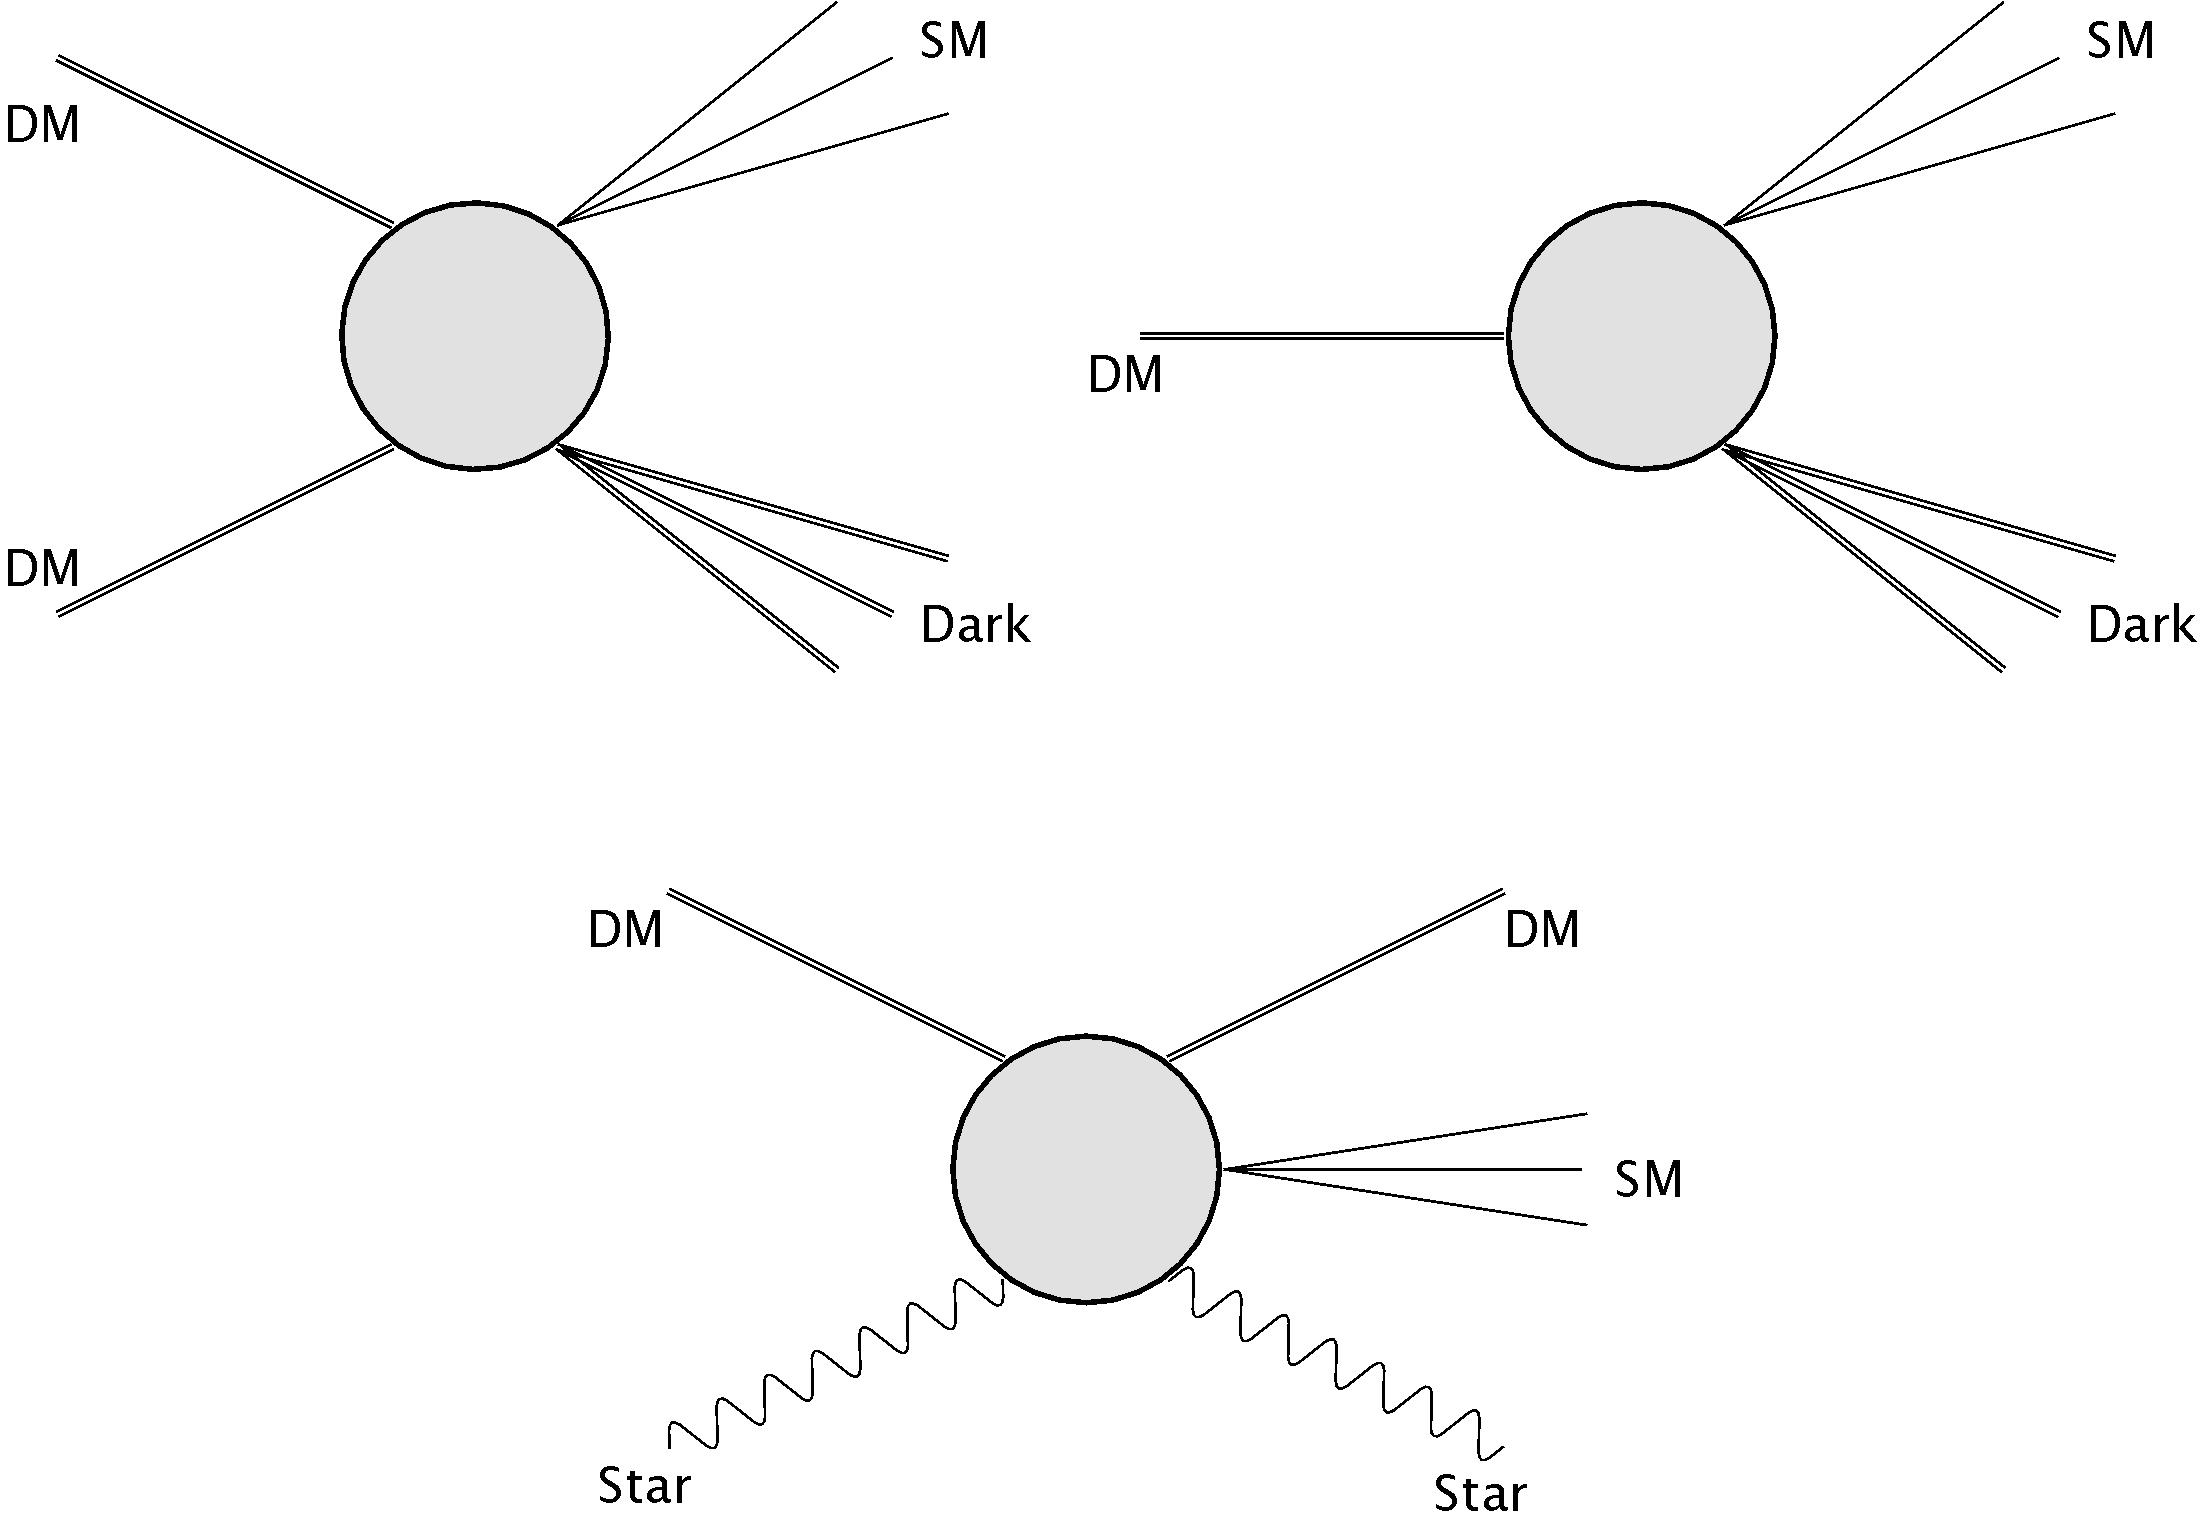
\includegraphics[scale=0.09]{feynmandiag.jpg}
\caption{Schematic of possible non-gravitational DM interactions in a WD. Heating of the WD occurs through SM particle production (also depicted are potential dark sector states involved).}
\label{fig:feynman}
\end{figure}

\subsection{DM-DM Collisions and DM Decays}
\label{sec:DMcoldecay}

The collision of two DM states or the decay of a single DM within the WD is a generic interaction found in many models.
Note that these DM-DM collisions are not necessarily particle-antiparticle annihilations, but can be of a more general, complicated nature such as the collisions of heavy nuclei.
Since any such event will likely result in both SM and dark sector products, we assume the energy released into the SM is a fraction $f$ of the DM mass.
Generically we might expect $f \ll 1$, although $f$ is at most unity for non-relativistic DM.
For simplicity, we only consider ``point-like" annihilations and decays which release SM particles within a sufficiently localized region. 
This excludes interactions involving the decay of long-lived, meta-stable dark states, i.e. displaced vertices. 
With this parameterization, the explosion condition is approximately the same for both DM-DM collisions and DM decays:
\begin{equation}
\label{eq:coldecay}
   m_\text{DM} \gtrsim \Eboom \cdot \frac{1}{f}
      \text{max}\left\{1, \frac{L_0}{\lambda_T}\right\}^3
\end{equation}

\subsection{DM Transits}
\label{sec:DMdecay}

For DM models with a DM-SM scattering interaction, there may be a continuous release of high-energy SM particles as the DM traverses a WD.
Since the DM will carry the bulk of the momentum in any such interaction producing light, relativistic SM secondaries, we can assume that the momentum of the released particles is isotropic.
This is parameterized by a linear energy transfer $(dE/dx)_\text{LET}$, which is the energy released into SM products per distance traveled in a WD.
Such a process can be broken up into a series of multiple heating events depositing energy $L_0 (d E/d x)_\text{LET}$ into temperature peaks of size $L_0$, where $L_0$ is the heating length for a single scatter. 
If any individual deposition satisfies \eqref{eq:boom}, then runaway fusion obviously occurs.
If not, a SN may still be triggered due to the combined effect of many deposits.
In such a scenario a large number of nearby temperature peaks will each diffuse outward, eventually merging into an explosive thermal profile satisfying \eqref{eq:boom}.
This is possible if the heating length is smaller than the trigger size $L_0 < \lambda_T$, in which case it is sensible to consider the combined deposit as a single heating event of length $\lambda_T$ and energy $\lambda_T (d E/d x)$.
However, such a coherent addition of individual energy deposits is only possible if the DM transit time is smaller than the relevant thermal evolution timescale.
The latter is dominated by the diffusion time $\tau_d$ across a distance $\lambda_T$ at temperature $T_f$.
Thus we require
\begin{align}
\tau_d \sim \frac{\lambda_T^2}{\alpha(T_f)} \gg \frac{\lambda_T}{v_\text{esc}},
\label{eq:SlowDiffusion}
\end{align}
where $\alpha(T_f)$ is the temperature-dependent diffusivity.
This condition is independent of DM model and has been checked to be satisfied for all WD densities.

In addition, we can parametrize the DM kinetic energy loss per distance travelled in a WD by a DM stopping power $(dE/dx)_\text{SP}$. 
Note that while $(dE/dx)_\text{LET}$ and $(dE/dx)_\text{SP}$ are conceptually related parameters and may be equal in important special cases, they are generically different.
We restrict ourselves to a ``bullet-like" transit in which DM penetrates the non-degenerate crust of a WD with negligible change in kinetic energy
\begin{align}
\label{eq:CrustCondition}
  \left( \frac{d E}{d x} \right)_\text{SP} \ll 
  \frac{m_\text{DM} v^2_\text{esc}}{R_\text{crust}},
\end{align}
where $R_\text{crust} \sim 50 ~\text{km}$ is the width of a WD crust and $v_\text{esc} \sim 10^{-2}$ is the escape velocity of a WD. 
If \eqref{eq:CrustCondition} were not satisfied, then the explosiveness of a transit would be highly dependent on details of the DM stopping power and must be calculated from a specific model.
We avoid this complexity by simply imposing that the DM reaches the degenerate stellar interior, where runaway fusion can be triggered, unimpaired in its initial transit of the star. 
Furthermore, note that $R_\text{crust}$ is many orders of magnitude larger than $\lambda_T$ or any of the heating lengths considered in this work. 
Therefore, the assumption of a DM transit at roughly constant velocity also allows us to ignore DM energy loss within the desired heating region in the WD interior. 
The explosion condition for transits satisfying \eqref{eq:SlowDiffusion} and \eqref{eq:CrustCondition} is given by
\begin{equation}
\label{eq:transitexplosion}
  \left( \frac{d E}{d x} \right)_\text{LET} \gtrsim n_\text{ion} T_f\, \text{max}\left\{\lambda_T, L_0 \right\}^2.
\end{equation}

\section{Dark Matter-Induced Ignition: Constraints}
\label{sec:Constraints}

We now constrain models of DM which will ignite a WD via one of the processes parameterized in Section \ref{sec:DMexplode}.
In order to do so, we additionally assume a simple, schematic form for the DM interactions such that $L_0$ can be calculated exactly. 
However, we first review the different ways in which white dwarfs can constrain DM candidates capable of triggering SN. 

\subsection{Review of WD Constraints}
Following the discussion of \cite{Graham:2015apa}, our constraints come from (1)~the existence of heavy, long-lived white dwarfs, or (2)~the measured type Ia SN rate. 
The typical age of a WD is of order the age of the universe $\sim \text{Gyr}$.
RX~J0648.04418 is a nearby star and one of the heaviest known WDs with a mass $\sim 1.25 ~M_{\odot}$. 
Of course, this is not the only known heavy WD - the Sloan Digital Sky Survey has found $\sim 20$ others. 
The NuStar collaboration has also recently uncovered evidence for the likely existence of $\sim 1.25 ~M_{\odot}$ WDs in the galactic center as well \textcolor{blue}{cite}.
Such candidates are particularly suited for our constraints as the energy deposit necessary to trigger SN $\Eboom$ is a decreasing function of WD mass. 
However, less dense white dwarfs are significantly more abundant in the galaxy.
Thus, even if a sufficiently massive DM is unable to trigger a violent heating event within the lifetime of a WD, it could still ignite enough lighter WDs to affect the measured SN rate of $\sim $ 0.3 per century.
The DM-induced SN rate is estimated using the expected number of white dwarfs per galaxy $\sim 10^{10}$ and their mass distribution \textcolor{blue}{cite}.
Simulations indicate that only WD masses heavier than $\sim 0.85 ~M_{\odot}$ will result in optically visible SN.
Therefore, most of the stars exploded in this manner will be in the mass range $\sim 0.85 - 1 ~M_{\odot}$, resulting in weaker SN than expected of typical Chandrasekhar mass WDs.

To summarize, a bound on DM parameters can be placed if either a single explosive event occurs during the lifetime of an observed star such as RX~J0648.04418, or the SN rate due to such DM events throughout the galaxy exceeds the measured value.
Note that for low-mass WDs dominated by photon diffusion, $\Eboom$ is a strong function of WD density. 
In \cite{Graham:2015apa} the central WD density is used to constrain black hole transits with the justification that the density is nearly constant for much of the star.
However, it is found that the WD density changes by an $\OO(1)$ fraction from the central value out at a distance $\sim R_\text{WD}/2$ \cite{Chandrasekhar}. 
Therefore the central density is a valid approximation as long as we consider heating events within this ``modified" WD volume. 
For simplicity, we employ this approach.  


\subsection{Collision and Decay Constraints}
\label{sec:CollisionConstraints}

The number of DM particles contained in a WD volume is approximately $\sim n_\text{DM} R_\text{WD}^3 (v_\text{esc}/v)$, taking into account the gravitationally enhanced DM number density within the star.
$v \sim 10^{-3}$ is the virial velocity of DM.
\textcolor{red}{of same order in galactic center?} Therefore, the expected DM-DM collision rate parameterized by cross-section $\sigma_\text{DM-DM}$ is 
\begin{equation}
\Gamma_\text{collision} \sim \l \frac{\rho_{\text{DM}}}{m_\text{DM}} \r^2 \sigma_\text{DM-DM} \l \frac{v_\text{esc}}{v}\r^3 v R_\text{WD}^3,
\label{eq:collisiongamma}
\end{equation}
where $\rho_{\text{DM}}$ is the energy density of DM in the region of interest.
For a nearby star we take $\rho_\text{DM} \sim 0.4 ~\GeV/\text{cm}^3$, while for the white dwarfs observed in the galactic center we assume $\rho_\text{DM} \sim 10^3 ~\text{GeV}/\text{cm}^3$.
Likewise, the rate at which a single DM decay event occurs in the WD is
\begin{equation}
\Gamma_\text{decay} \sim  \frac{1}{\tau_\text{DM}} \frac{\rho_{\text{DM}}}{m_\text{DM}} \l \frac{v_\text{esc}}{v} \r R_\text{WD}^3,
\label{eq:taugamma}
\end{equation}
where $\tau_\text{DM}$ is the mean lifetime of DM.

We are able to constrain DM parameters whenever such processes satisfy the explosion condition $\eqref{eq:coldecay}$. 
Consider a schematic interaction where an annihilation or decay releases a number of SM particles $N$ of single species $i$ and individual energy $\epsilon$. 
These released particles will deposit their energy and thermalize ions within a heating length explicitly calculated in Section \ref{sec:SMHeating}. 
If we assume a fractional parameter $\eta=1$, this corresponds to the entire mass of DM being converted into SM particles $i$, each with energy $m_\text{DM}/N$.
At sufficiently large $\epsilon \gtrsim \text{TeV}$, it has been shown that the heating properties for most SM species only varies logarithmically in energy.
Therefore, we treat $\epsilon$ as a free parameter whose precise value above $\sim \text{TeV}$ does not qualitatively modify the limits imposed.
In this case, $N$ and $\epsilon$ can both be fixed to the value at which $N \epsilon$ is of order $m_\text{DM}$ without affecting the nature of the constraints.
%The only caveat in this scenario is that the value of $L_i (\epsilon)$ extrapolated to energies beyond $\sim 10^{17} ~\GeV$ must be done with caution.
%As a result, for $m_\text{DM}$ greater than this scale, one can simply impose $\epsilon \lesssim 10^{17} ~\GeV$ with the number of released particles necessarily $N > 1$.
With the above schematic for DM-DM collisions, we constrain the cross-section $\sigma_\text{DM-DM}$ as a function of $m_\text{DM}$ using the different classes of observation available and for representative choices of $\eta$ and SM species $i$ released.
This is done in Figures \ref{fig:collisionclasses}, \ref{fig:collisioneta}, and \ref{fig:collisionspecies}. 
In a similar manner, we constrain the lifetime $\tau_\text{DM}$ as a function of $m_\text{DM}$ in Figures \ref{fig:decayclasses}, \ref{fig:decayepsilon}, and \ref{fig:decayspecies}.

\begin{figure}
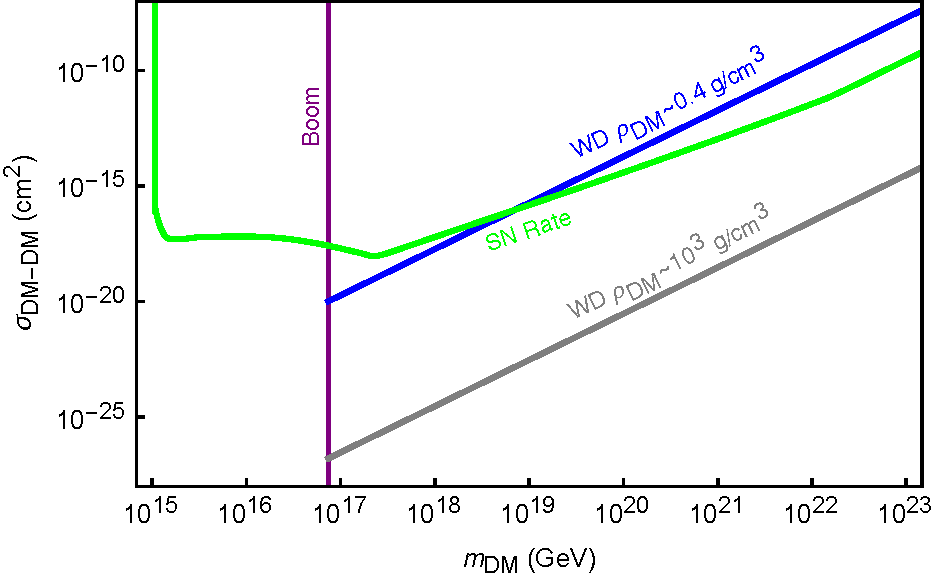
\includegraphics[scale=.45]{collisionobservation.pdf}
\caption{Constraints on DM-DM collision cross-section into photons with $\eta =1$. Bounds come from observations of a single WD (local and galactic center) and measured SN rate}
\label{fig:collisionclasses}
\end{figure}

\begin{figure}
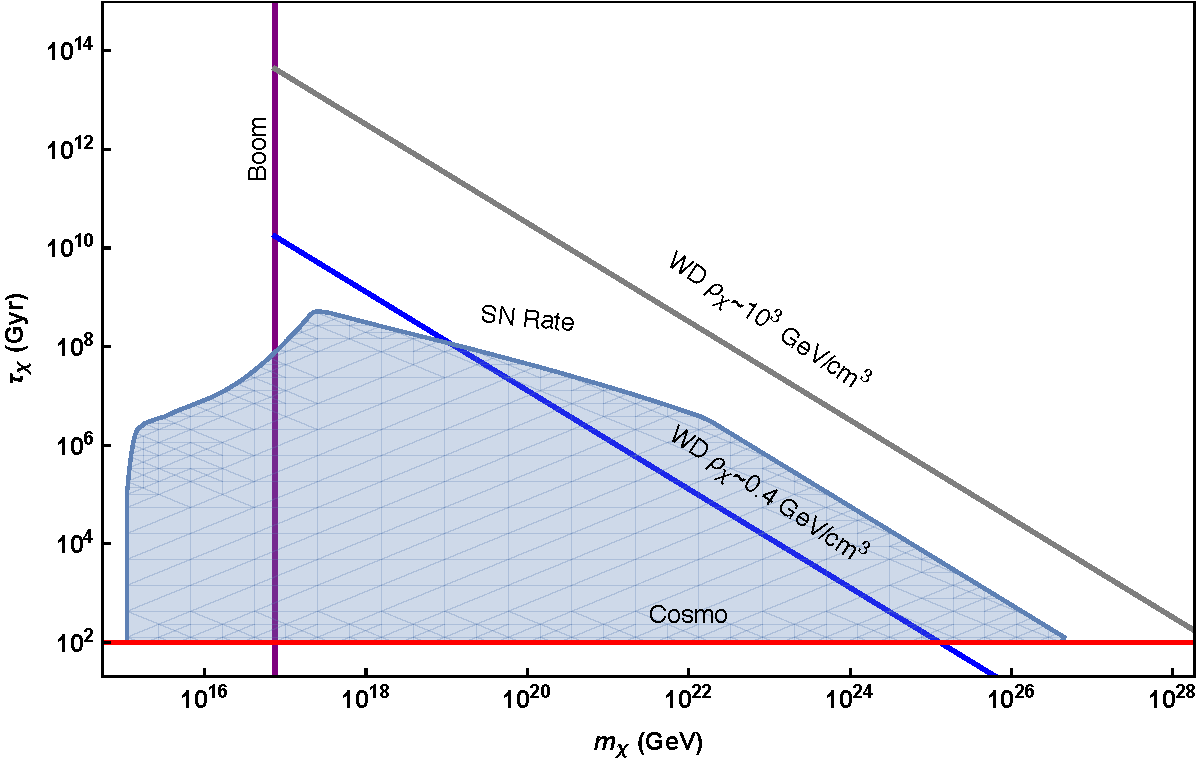
\includegraphics[scale=.45]{decayobservation.pdf}
\caption{Constraints on DM decay lifetime into photons with $\eta =1$. Bounds come from observations of a single WD (local and galactic center) and measured SN rate}
\label{fig:decayclasses}
\end{figure}
 
\subsection{Transit Constraints}
\label{sec:TransitConstraints}

The DM transit rate through a WD (including a gravitational Sommerfeld enhancement) is given by
\begin{align}
\Gamma_\text{transit} \sim \frac{\rho_{\text{DM}}}{m_\text{DM}} R_\text{WD}^2 \l\frac{v_\text{esc}}{v}\r^2 v.
\label{eq:TransitFluxCondition}
\end{align}
In order to constrain a DM model through its transit interaction with a WD, we require that it satisfy the explosive condition \eqref{eq:transitexplosion}. 
This is given in terms of an LET, which parameterizes the ability for DM to release sufficient energy to the star in the form of SM particles.
$(dE/dx)_\text{LET}$ for any realistic DM model would necessarily involve a sum over stellar targets along with species that could be produced, as well as an integral over the produced particle spectrum.
However, consider a simplified interaction in which $\sigma_{i,\epsilon}$ denotes the cross-section for DM to scatter off a stellar constituent, producing $N$ particles of species $i$ and each with energy $\epsilon$.
If this were the only available channel for the DM to deposit energy, then its LET could be written as
\begin{align}
\label{eq:schematicLET}
  \left( \frac{d E}{d x} \right)_\text{LET} = n_\text{ion} \cdot N \sigma_{i,\epsilon} \epsilon,
\end{align}
where we now specify to the case of DM collisions with nuclear targets. 
With such a schematic for the DM-SM scattering interaction, the transit heating length for the process can be explicitly calculated using the results of Section~\ref{sec:SMHeating}.

In addition, we also make a sensible assumption that the LET $(dE/dx)_\text{LET}$ and DM stopping power $(dE/dx)_\text{SP}$ are equal for fixed number density - that is, the DM loses kinetic energy at the same rate as energy is deposited to the WD.
While such a statement is certainly not true for all DM models (such as the Q-ball, which liberates binding energy rather than transferring kinetic energy), it provides a useful benchmark to express constraints.
With this assumption, it is interesting to note that combining the transit explosion condition \eqref{eq:transitexplosion} with $\eqref{eq:schematicLET}$ yields a lower bound on DM mass such that the DM is able to both penetrate the crust \emph{and} trigger an explosion:
\begin{align}
\label{eq:transitmass}
m_{\text{DM}} >  T_f \lambda_T^2 \l \frac{n_{\text{crust}} R_{\text{crust}}}{v_{\text{esc}}^2} \r.
\end{align}
For typical WD parameters we find that the DM mass must be greater than $\sim 10^{27} ~\GeV$, taking the density of the WD crust $n_\text{crust}$ to be a nominal $\OO(10^{-2})$ fraction of the central density $n_\text{ion}$ \cite{Chandrasekhar}. 
In other words, if \eqref{eq:transitmass} were violated then the DM interaction is either not strong enough to ignite the WD or is so strong that the DM cannot penetrate the crust without losing appreciable kinetic energy.
However, it is important to note that this bound is only applicable when the energy input to the WD is chiefly coming from the DM kinetic energy, rather than binding energy or other sources.
With the above schematic for a DM transit, we constrain the parameter $\sigma_{i,\epsilon}$ as a function of DM mass $m_\text{DM}$ - for simplicity, we take a single SM particle released per interaction $N = 1$. 
This is done in Figures \ref{fig:transitclasses}, \ref{fig:transitepsilon}, and \ref{fig:transitspecies} using the different classes of observation available and for representative choices of $\epsilon$ and SM species $i$ released.

\begin{figure}
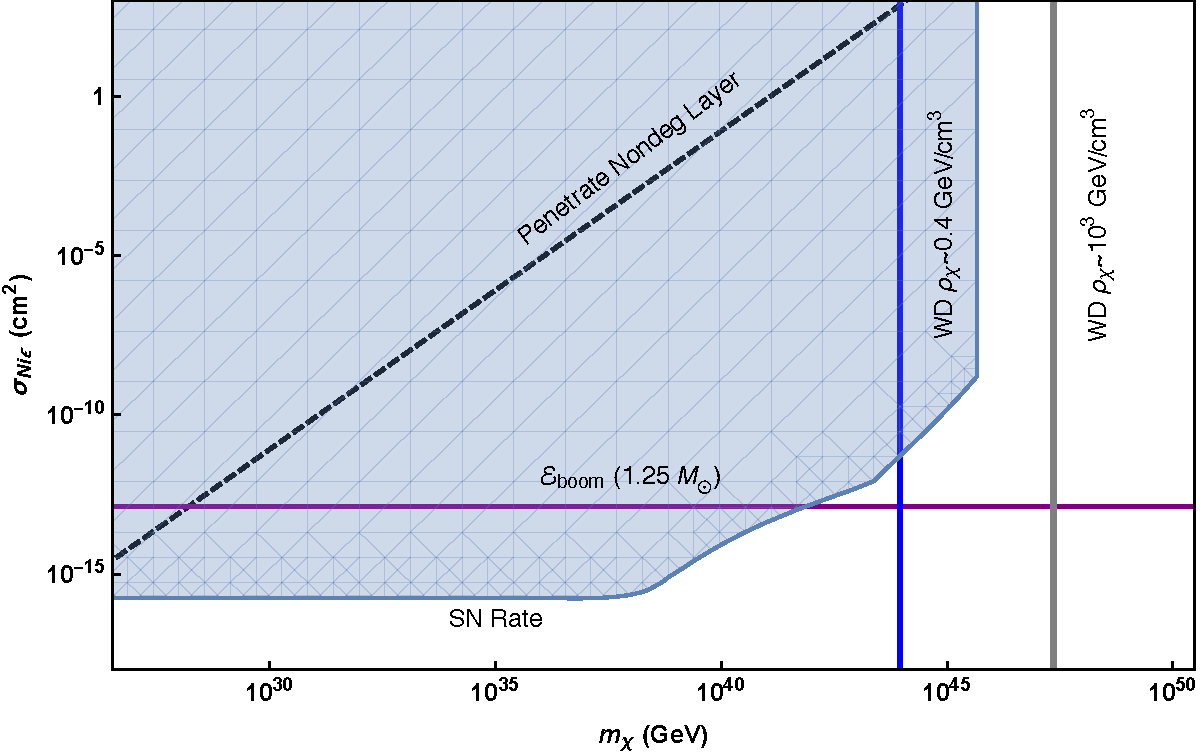
\includegraphics[scale=.45]{transitobservation.pdf}
\caption{Constraints on DM-nuclei scattering cross-section to produce photons of energy $\epsilon = \text{TeV}$. Bounds come from observations of a single WD (local and galactic center) and measured SN rate}
\label{fig:transitclasses}
\end{figure}

\section{Q-balls}
\label{sec:QBalls}

Having derived generic constraints on models of ultra-heavy DM in Section~\ref{sec:Constraints}, we turn towards a more concrete example: Q-balls.
In various supersymmetric extensions of the SM, non-topological solitons called Q-balls can be produced in the early universe \cite{Coleman:1985ki, Kusenko:1997si}.
If these Q-balls were stable, they would comprise a component of the DM today.
For gauge-mediated models with flat scalar potentials, the Q-ball mass and radius are given by
\begin{equation}
\label{eq:Qballprop}
M_Q \sim m_S Q^{3/4}, ~~~ R_Q \sim m_S^{-1} Q^{1/4},
\end{equation}
where $m_S$ is related to the scale of supersymmetry breaking.
The condition $M_Q/Q < m_p$ ensures that the Q-ball is stable against decay to nucleons \cite{Dine:2003ax}.
When an (electrically neutral) baryonic Q-ball interacts with a nucleon, it absorbs its baryonic charge as a minimum-energy configuration and induces the dissociation of the nucleon into free quarks.
During this proton decay-like process, $\sim \text{GeV}$ of energy is released through the emission of 2 - 3 pions \cite{Dine:2003ax}.
We assume that for each Q-ball collision, there is equal probability to produce $\pi^0$ and $\pi^\pm$ under the constraint of charge conservation.
The cross-section for this interaction is approximately geometric:
\begin{align}
\sigma_Q \sim \pi R_Q^2.
\end{align}
Note that a sufficiently massive Q-ball will become a black hole if the Q-ball radius is less than the Schwarzschild radius $R_Q \lesssim G M_Q$.
In the model described above, this translates into a condition $(M_\text{pl}/m_S)^4 \lesssim Q$.
For Q-ball masses of this order, gravitational interactions become relevant.

We now determine the explosiveness of a Q-ball transit. 
In the notation of Section \ref{sec:Constraints}, this process is described by the parameter $(dE/dx)_\text{LET} \sim n_\text{ion} \cdot N \sigma_Q \epsilon$, where the nuclear interaction results in $N \sim 30$ pions released, each with kinetic energy $\epsilon \sim 500 ~\text{MeV}$.
The Q-ball interaction is simple enough that the heating length of a Q-ball transit is computed in a straightforward manner $L_0 \approx 10^{-6} ~\text{cm}$ at a number density $n_\text{ion} \sim 10^{32}~\text{cm}^{-3}$. $L_0$ scales inversely with $n_\text{ion}$ and is less than $\lambda_T$ for all WD densities, so the Q-ball cross-section necessary to trigger runaway fusion is simply $\sigma_Q \gtrsim \lambda_T^2 (T_f/\epsilon) \approx 10^{-4} \lambda_T^2$.
If the Q-ball cross-section is related to its mass and baryonic charge as in \eqref{eq:Qballprop}, we find that $Q \gtrsim 10^{38} (m_S/\text{TeV})^4$ is capable of destroying a heavy $\sim 1.25 ~M_{\odot}$ WD.
Note that for such large values of $Q$ there is negligible stopping power for the Q-ball to slow down in a WD, and as such condition \eqref{eq:CrustCondition} will be trivially satisfied.
Currently, the strongest constraints on Q-balls come from Super-Kamiokande as well as air fluorescence detectors of cosmic rays.
However, the constraints possible with the WD detector are in a fundamentally inaccessible region of parameter space for these terrestrial-based experiments due to the extremely low flux, and thus our new constraints are wholly complementary.
The strongest proposed limits due to the existence of a heavy WD in the galactic center are plotted in Figure~\ref{fig:Qballconstraint}. As a comparison, the combined limits from Super-K and the OA,TA cosmic ray detectors are shown in red. 
\begin{figure}
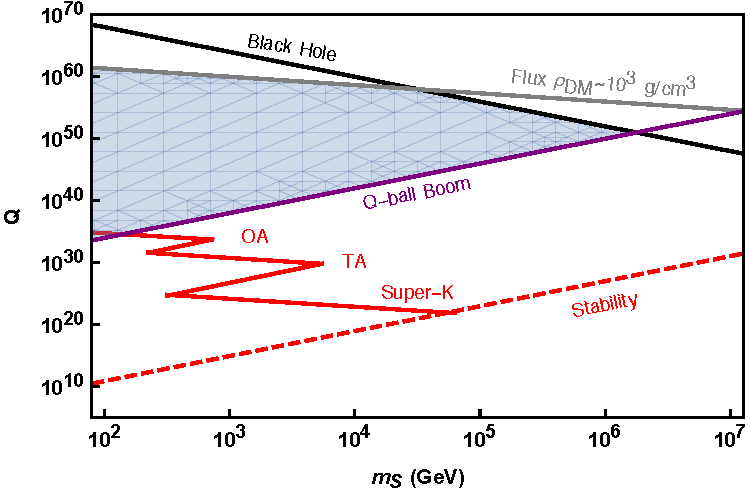
\includegraphics[scale=.55]{Qballconstraint.pdf}
\caption{Constraints on baryonic Q-balls from transits of a $\sim 1.25 ~M_{\odot}$ WD in the galactic center, $\rho_\text{DM} \sim 10^3 ~\text{g}/\text{cm}^3$. Also shown are the limits from Super-K and the OA, TA cosmic ray detectors.}
\label{fig:Qballconstraint}
\end{figure}

\section{Discussion}
\label{sec:Discussion}

\begin{appendices}

\section{Particle Interactions in a White Dwarf}
\label{sec:Appendix}
Here we provide a detailed analysis of the electromagnetic and strong interactions in a WD.
This is primarily aimed towards calculating the stopping of electrons, photons, and light hadrons (pions, protons, neutrons) within the stellar medium at energies greater than $\sim \text{MeV}$. 
These results of these stopping powers are summarized in Figures \ref{fig:SPelectron}, \ref{fig:SPphoton}, \ref{fig:SPnuc}, and \ref{fig:SPpion}.
Note that we will assume a carbon-oxygen WD.
The stellar medium is very dense, with electron and ion number densities in the range $n_e = Z n_\text{ion} \sim 10^{30} - 10^{33} ~\cm^{-3}$.  
This implies the efficient stopping of incident particles while also giving rise to qualitatively different effects than seen in terrestrial detectors.  
Famously, the star is supported against collapse by the relativistic electron degeneracy pressure with a characteristic Fermi energy
\begin{equation}
  E_F \sim (3 \pi^2 n_e)^{1/3} \sim 0.1 - 1 ~\MeV
\end{equation}
which is much larger than the typical stellar temperature $T \sim \keV$. 
The nuclei form a strongly-coupled plasma with Coulomb interaction energy
\begin{equation}
\label{eq:lattice}
  \omega \sim \frac{Z^2 \alpha}{n_\text{ion}^{-1/3}} 
         \sim 10^{-2} - 10^{-1} ~\MeV.
\end{equation}
Since it is generally the case that $\omega >T$, the ions form a Coulomb lattice with lattice binding energy $\sim \omega$. 
\begin{figure}
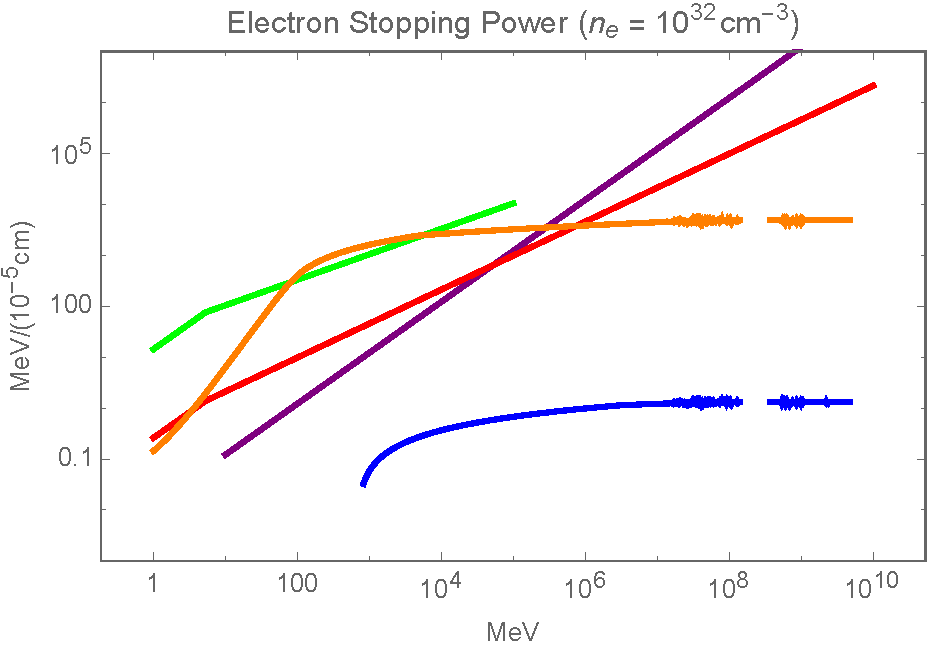
\includegraphics[scale=.60]{SPelectron.pdf}
\caption{Electron energy loss in a WD density $n_e = 10^{32} ~\text{cm}^{-3}$}
\label{fig:SPelectron}
\end{figure}

\begin{figure}
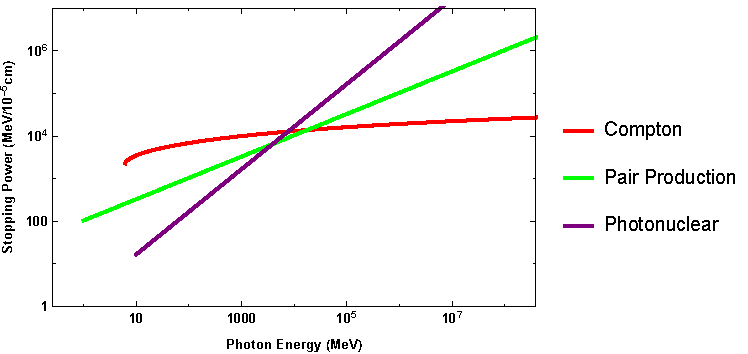
\includegraphics[scale=.60]{SPphoton.pdf}
\caption{Photon energy loss in a WD density $n_e = 10^{32} ~\text{cm}^{-3}$}
\label{fig:SPphoton}
\end{figure}

\begin{figure}
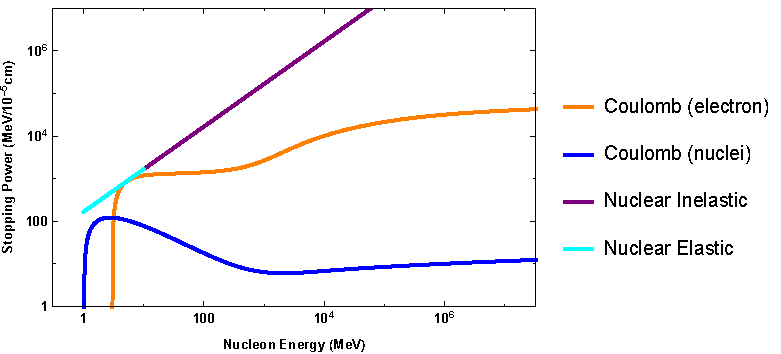
\includegraphics[scale=.60]{SPnucleon.pdf}
\caption{Nucleon energy loss in a WD with density $n_e = 10^{33} ~\text{cm}^{-3}$. The Coulomb stopping powers apply only to protons.}
\label{fig:SPnuc}
\end{figure}

\begin{figure}
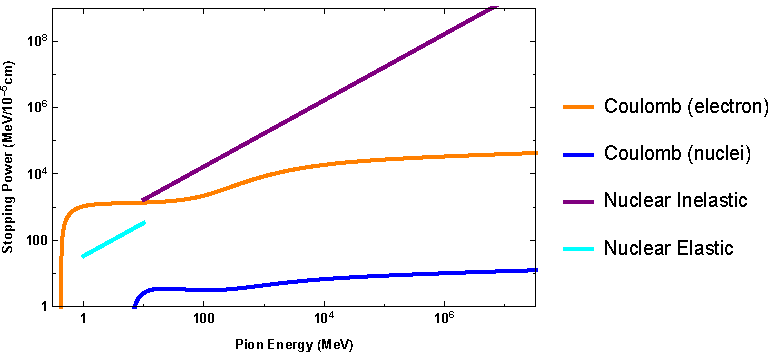
\includegraphics[scale=.60]{SPpion.pdf}
\caption{Pion energy loss in a WD with density $n_e = 10^{33} ~\text{cm}^{-3}$. The Coulomb stopping powers apply only to charged pion.}
\label{fig:SPpion}
\end{figure}

\subsection{Coulomb Collisions}
%Elastic electromagnetic interactions are a dominant source of energy loss for low-energy charged particles scattering off both ions and degenerate electrons in the WD. 
A particle of mass $m$, charge $e$, and velocity $\beta$ incident on a stationary target of mass $M$ and charge $Ze$ will transfer an energy $W$ as given by the (recoilless) Mott cross-section 
\begin{equation}
  \frac{d \sigma}{dW} = \frac{2 \pi \alpha^2 Z^2}{M \beta^2} \frac{1}{W^2} 
    \l 1-\beta^2 \frac{W}{W_\text{kin}} \r,
\label{eq:mott}
\end{equation}
and we have assumed a sufficiently fast incident particle so that interactions are governed by single collisions with energy transfer $W$ \cite{Agashe:2014kda}.
$W_\text{kin}$ is the maximum possible energy transfer satisfying kinematic constraints (i.e., a backward scatter)
\begin{equation}
\label{eq:ekin}
  W_{\text{kin}} = \frac{2 M \beta^2 \gamma^2}{1+ 2\gamma M/m +(M/m)^2}.
\end{equation}
%The stopping power due to Coulomb scatters is then given by 
%\begin{equation}
%\label{eq:sp-general}
%    \frac{dE}{dx} = \int n_\text{target} W \l \frac{d \sigma}{dW} \r dW,
%\end{equation}
%where $n_\text{target}$ is the number density of target particles.
For a heavy particle incident on an electron target this reduces to $W_\text{kin} \approx 2 m_e \beta^2 \gamma^2$, while for electron-electron scattering we take $W_\text{kin}$ to be half the energy of the incident electron to account for the identical particles \cite{jackson_classical_1999}.
It is straightforward to understand the parametric dependences of \eqref{eq:mott}: there is increased likelihood to scatter for slowly moving incident particles undergoing soft-scatters against lighter targets.

We first compute the energy loss for scattering off nuclear targets.
In this case, the Coulomb stopping power is parametrically of order
\begin{align}
\label{eq:SP}
  - \l \frac{dE}{dx}\r \sim \frac{n_\text{ion} Z^2 \alpha^2}{M \beta^2} 
    \log {\l\frac{W_\text{kin}}{W_\text{min}}\r}.
\end{align}
The minimum energy transfer here is set by either charge screening or lattice effects.  
In a WD, the screening length $\kappa_{\text{sc}}^{-1}$ due to the degenerate electron gas can be calculated in the Thomas-Fermi approximation \cite{Teukolsky}
\begin{equation}
\label{eq:TF}
\kappa_{\text{sc}}^{2} = \frac{6 \pi Z \alpha n_e}{E_F}.
\end{equation}
To estimate the energy transfer at this screening length, we use the fact that a soft Coulomb scatter at impact parameter $b$ will transfer energy of order
\begin{equation}
\label{eq:impact}
  W \sim \frac{Z^2 \alpha^2}{b^2 \beta^2 M}.
\end{equation}
In addition, for energy transfers less than the ion lattice energy $\omega$, the lattice structure of ions must be taken into account. 
In particular, energy transfers below this threshold will occur via the creation of phonon excitations and will be suppressed from the free-particle results used above. 
%We thus take the lower bound for energy transfer via free-particle Coulomb scattering off nuclear targets to be $\text{Max}\{W_\text{sc},~\omega\$.
%If $W_\text{TF} < \omega$, we estimate the stopping power for small energy transfers, $W < \omega$, by \textcolor{blue}{paragraph on phonons}. 

Now consider Coulomb collisions with electrons targets. 
The cross-section \eqref{eq:mott} is no longer fully valid -  must account for a significant target recoil as well as identical particle effects in the case of electron-electron scattering (i.e., the M{\"o}ller cross-section).
One would also need to average over the relativistic motion of the degenerate electrons. 
However, after integrating to find the stopping power, we find these are only $\OO(1)$ corrections. 
The electron degeneracy now plays a significant role, as an incident particle transferring energy $W$ can only scatter electrons within $W$ of the Fermi surface.
We account for this with a modified density of target electrons:
\begin{equation}
\label{eq:pauliblocking}
  n_e \l W \r = 
  \begin{cases}
    \displaystyle \int \limits_{E_F - W}^{E_F} dE ~g(E), &  W < E_F  \\
    \quad             n_e                                &  W > E_F,
  \end{cases}
\end{equation}
where $g(E)$ is the density of states per unit volume of a three-dimensional free electron gas.
Therefore, unlike in the non-degenerate case, the energy loss due to soft-scatters are in fact subdominant to the contributions from rare hard-scatters due to Pauli-suppression.
We additionally demand that the incident electron remains above the Fermi energy after scatting, that is $W < E - E_f$. 
This yields a stopping power that is roughly constant at high energies:
\begin{equation}
-\l \frac{dE}{dx} \r \sim \frac{n_e \alpha^2}{m_e},
\end{equation}
and which vanishes abruptly as the incident energy $E$ approaches the Fermi energy. 

\subsection{Compton and Inverse Compton Scattering}

Photons and charged particles can elastically exchange energy through Compton scattering.
We focus first on an incident photon losing energy to the WD medium.
Since the cross-section for this process scales inversely with the target mass, the stopping due to photon-ion collisions will be far subdominant to photon-electron collisions and we ignore the former. 
Consider an incident photon of energy $k$ scattering off an electron of energy $\sim E_F$.
In the rest frame of the electron, this cross-section is given by the Klein-Nishina formula
\begin{equation}
\label{KN}
  \frac{d\sigma_\text{KN}}{d (\cos \theta)} = \frac{\pi \alpha^2}{m_e^2} 
  \l \frac{k^\prime}{k} \r^2 
  \l \frac{k^\prime}{k} + \frac{k}{k^\prime} -\sin^2 \theta \r
\end{equation}
where $k^\prime$ is the outgoing photon energy, related to the scattering angle $\theta$ by the Compton formula
\begin{equation}
{k^{\prime }={\frac {k}{1+{\frac {k}{m_e}}(1-\cos \theta )}}}.
\end{equation}
In the limit $k > m_e$, the cross-section is suppressed by the incoming energy $\sigma_\text{KN} \sim \frac{\alpha^2}{m_e k}$. 
The outgoing photons will scatter predominately in a near-forward direction $\cos \theta \approx m_e/k$ so that $k^\prime \sim m_e$.
Thus the typical photon energy loss is large, and cooling proceeds via a small number of hard scatters.
The Compton stopping power is estimated to be
\begin{equation}
\label{eq:approx-comptonSP}
  - \l\frac{dk}{dx}\r \sim \frac{n_e \alpha^2}{m_e} \l 1 - \frac{m_e}{k} \r.
\end{equation}
A more detailed analysis computes the stopping power as 
\begin{equation}
\label{eq:comptonSP}
  -\l\frac{dk}{dx}\r =  \int d (\cos \theta) n_e \frac{d\sigma_\text{KN}}{d (\cos \theta)} \l k - k^\prime \r,
\end{equation}
with an appropriate Lorentz boost to the electron rest frame, although the full result only differs from the above estimate by $\OO(1)$ factors.
Further, Pauli-blocking of the target electrons should be taken into account using a modified number density as in \eqref{eq:pauliblocking}.
We find that degeneracy only introduces a significant suppression when $k \lesssim 10 ~\text{MeV}$, which is to be expected since the interaction is dominated by hard, near-forward scatters.

We now briefly consider incident electrons which may cool by (inverse) Compton scatters with the thermal bath of photons in the WD.  
The number density of these photons is set by the temperature of the star $n_\gamma \sim T^3 \sim 10^{23} ~\cm^{-3}$, where we have taken $T \sim \text{keV}$. 
As this is parametrically smaller than the number density of electrons, it is reasonable to suspect that the energy loss due to inverse Compton scattering is far subdominant to electron-electron collisions.
An estimate in the manner of \eqref{eq:approx-comptonSP} gives the inverse Compton stopping power in terms of the photon temperature $T$ and incident electron energy $E$ 
\begin{equation}
\label{eq:invcomptonSP}
  -\l \frac{dE}{dx}\r \sim 
  \begin{cases}
    \alpha^2 \frac{T^4}{m_e^4} E^2 & E \lesssim \frac{m_e^2}{T} \\
    \alpha^2 T^2 & E \gtrsim \frac{m_e^2}{T} \\
  \end{cases},
\end{equation}
where the change in scaling with $E$ marks a transition from Thompson-like scattering in the electron rest frame to suppressed high-energy scattering.
As expected, we find that the inverse Compton stopping power is negligible compared to Coulomb scattering. 

\subsection{Bremsstrahlung and Pair Production with LPM Suppression}
Bremsstrahlung and pair production should also be considered as stopping mechanisms for high-energy electrons and photons. We restrict our attention to radiative processes off target nuclei rather than target electrons as the latter are additionally suppressed by degeneracy, kinematic recoil, and charge factors. 
The cross-section for an electron of energy $E$ to radiate a photon of energy $k$ is given by the Bethe-Heitler formula
\begin{equation}
\label{eq:BH}
\frac{d \sigma_\text{BH}}{dk} = \frac{1}{3 k n_\text{ion} X_0} (y^2+2 [1+ (1-y)^2]), ~~~ y = k/E.
\end{equation}
$X_0$ is the radiation length, and is generally of the form
\begin{equation}
\label{eq:radiationlength}
X_0^{-1} = 4 n_\text{ion} Z^2 \frac{\alpha^3}{m_e^2} \log{\Lambda}, ~~~ \log{\Lambda} \sim \int \limits_{b_\text{min}}^{b_\text{max}} \frac{1}{b}.
\end{equation}
where $\log{\Lambda}$ is a logarithmic form factor containing the maximum and minimum effective impact parameters allowed in the scatter.
Integrating \eqref{eq:BH}, we find the energy loss due to bremsstrahlung is simply 
\begin{equation}
-\l\frac{dE}{dx}\r \sim \frac{E}{X_0}.
\end{equation}
$b_\text{min}$ in \eqref{eq:radiationlength} is set by a quantum-mechanical bound such that the radiated photon frequency is not larger than the initial electron energy. 
For a bare nucleus, this distance is the electron Compton wavelength $b_\text{min} \sim \frac{1}{m_e}$. \textcolor{blue}{another sentence to clarify?}
It is important to note that collisions at impact parameters less than $b_\text{min}$ will still radiate, but with suppressed intensity.
Classically, this is manifested by the decoherence of radiation at large scattering angles.
$b_\text{max}$ is set by the distance at which the nuclear target is screened.
For an atomic target this is of order the Bohr radius, and for nuclear targets in the WD this is the Thomas-Fermi screening radius given by \eqref{eq:TF}.
Evidently, there exists a critical electron number density $n_e \sim 10^{32} ~\text{cm}^{-3}$ when the logarithmic form factor appears to vanish. 
For our purposes, we simply take $\log{\Lambda} \sim \OO(1)$ for all WD densities under consideration and refrain from a full quantum-mechanical calculation at small impact parameters. 
%For our purposes, we simply take $\log{\Lambda} \sim \OO(1)$ whenever $b_\text{min} \lesssim b_\text{max}$ while effectively ignoring the energy loss due to bremsstrahlung in a sufficiently dense WD.

However, bremsstrahlung will be suppressed by the ``Landau-Pomeranchuk-Migdal" (LPM) effect - see \cite{Klein:1998du} for an extensive review.
High-energy radiative processes involve very small longitudinal momentum transfers to nuclear targets ($\propto k/E^2$ in the case of bremsstrahlung).
Quantum mechanically, this interaction is delocalized across a formation length over which amplitudes from different scattering centers will interfere.
This interference turns out to be destructive and must be taken into account in the case of high energies or high-density mediums.
Calculations of the LPM effect can be done semi-classically based on average multiple scattering.
It is found that bremsstrahlung is suppressed for $k < E(E-k)/E_\text{LPM}$, where
\begin{equation}
\label{eq:LPM}
E_\text{LPM} = \frac{m_e^2 X_0 \alpha}{4 \pi}.
\end{equation}
For the WD densities in which radiative energy loss is considered, $E_\text{LPM} \sim 10-10^{3} ~\text{MeV}$.
The degree of suppression is found to be
\begin{equation}
\frac{d\sigma_\text{LPM}/dk}{d\sigma_\text{BH}/dk} = \sqrt{\frac{k E_\text{LPM}}{E (E-k)}},
\end{equation}
so that the bremsstrahlung stopping power in the regime of high-suppression is modified
\begin{equation}
\label{eq:bremloss}
-\l\frac{dE}{dx}\r_\text{LPM} \sim \l\frac{E_\text{LPM}}{E} \r^{1/2} \frac{E}{X_0}, ~~~ E>E_\text{LPM}.
\end{equation}
We find that the LPM effect diminishes energy loss due to soft radiation so that the radiative stopping power is dominated by single, hard bremsstrahlung.

In addition to the LPM effect, other forms of interaction within a formation length will suppress bremsstrahlung when $k \ll E$.
The emitted photon can coherently scatter off electrons and ions in the media, acquiring an effective mass of order the plasma frequency $\omega_p$.
Semi-classically, this results in a suppression of order $(k/\gamma \omega_p)^2$ when the radiated photon energy $k < \gamma \omega_p$.
This is known as the ``dielectric effect".
For high-energy electrons, this dielectric suppression only introduces a minor correction to \eqref{eq:bremloss}, in which soft radiation is already suppressed by the LPM effect \cite{Klein:1998du}.

We now briefly summarize the stopping of photons via pair production. Similar to \eqref{eq:BH}, the cross-section for a photon of energy $k$ to produce an electron-positron pair with energies $E$ and $k-E$ is
\begin{equation}
\label{eq:PP}
\frac{d \sigma_\text{BH}}{dE} = \frac{1}{3 k n_\text{ion} X_0} (1+ 2[x^2+ (1-x)^2]) ~~~ x = E/k,
\end{equation}
valid beyond the threshold energy $k \gtrsim m_e$. 
As a result, the pair production cross-section $\sim 1/(n_\text{ion} X_0)$.
However, the LPM effect suppresses pair production at energies $E(k-E) > k E_\text{LPM}$ so that the cross-section reduces to
\begin{equation}
\sigma_{pp} \sim \l\frac{E_\text{LPM}}{k} \r^{1/2} \frac{1}{n_\text{ion} X_0}, ~~~ E>E_\text{LPM}.
\end{equation}
Note that the LPM effect is less significant for higher-order electromagnetic processes since these generally involve larger momentum transfers for the same final-state kinematics.
Thus, when the suppression factor exceeds $\OO(\alpha)$, these interactions should also be considered.
For instance, the energy loss due to electron direct pair production $eN \to e^+ e^- e N$ has been calculated in \cite{Gerhardt:2010bj} and is found to exceed that of bremsstrahlung at an energy $\sim 10^{8} ~\GeV$. 
A similar crossover is to be expected for other higher-order diagrams as well, although such a calculation is beyond the scope of this work. 
Rather, it is expected that at such high energies the stopping power is dominated by photonuclear and electronuclear interactions anyway, and we may simply ignore the contributions from other radiative processes \textcolor{blue}{cite convo with Klein}. 

\subsection{Nuclear Interactions}
Finally, we discuss particle interactions in the WD due the strong force. 
Nuclear interactions can be either elastic or nonelastic - the nature of the interaction is largely determined by the incident particle energy. 
Elastic collisions are most relevant for energy loss at scales less than the nuclear binding energy $\sim 10 ~\text{MeV}$.
A single, backward elastic scatter could result in an incident particle losing virtually all of its energy if the incident and target masses are the same.
However, we will be primarily concerned with light hadrons incident on relatively heavy nuclei, i.e. ping-pong balls bouncing around a sea of bowling balls.
An elastic collision between a incident, non-relativistic hadron of mass $m$, kinetic energy $E$ and a stationary nuclear target of mass $M$ results in an average final energy
\begin{equation}
\label{eq:elasticratio}
E' \sim \l \frac{m}{M}\r E, ~~~~ m < M,
\end{equation}
where it is assumed there is an isotropic distribution in the center-of-mass scattering angle.
Thus a nucleon interacting with carbon nuclei on average transfers 15\% of its incident energy after each elastic collision.
At high-energies, the cross-section for elastic scatters $\sigma_\text{el}$ is more or less independent of the incident particle species and energy.
Above $\sim \text{MeV}$, electrostatic repulsion is negligible for nuclear interactions of protons and $\pi^+$. 
Therefore, the stopping power due to elastic collisions is of the form
\begin{equation}
- \l \frac{dE}{dx} \r \sim \l \frac{m}{M} \r \frac{E}{l_\text{el}}, ~~~~ l_\text{el} \sim \frac{1}{n_\text{ion} \sigma_\text{el}}.
\end{equation}
$l_\text{el}$ denotes the mean free path for elastic collisions. 
Above $10 ~\MeV$ the cross section for nuclear elastic collisions is approximately the geometric cross section of carbon nuclei $\sim 100 ~\text{mb}$, while at $\MeV$ energies the elastic cross section generally rises to be of order $\sim \text{b}$. 
The interaction in the intermediate regime $1 - 10 ~\MeV$ is dominated by nuclear resonances and is of a complicated form. 
For our purposes, we will simply take the elastic cross section for nucleons and pions to be $\sigma_\text{el} \approx 100~\text{mb}$ when $E \gtrsim 10 ~\MeV$ and $\sigma_\text{el} \approx \text{b}$ when $E \lesssim 10 ~\MeV$. 

Next we consider inelastic collisions for hadron incident energies greater than the nuclear binding energy $\sim 10 ~\MeV$.  
In such a collision the target nucleus is broken up and the nuclear fragment is typically in an unstable state.  
The relaxation process occurs in a number of steps and proceeds primarily through the slow emission of low-energy hadrons and photons.
The incident hadron will also will also undergo a violent collision with one or more nucleons in the 
a violent collision with one or more protons or neutrons in the nucleus. In this collision
a number of additional hadrons is produced 
For incident energies are greater than the nuclear binding energy $\sim \GeV$, the interaction produces an $\OO(1)$ number of hadrons which roughly carry the initial energy. 
Above the pion

These secondary particles approximately split the initial total energy of the absorbed primary particle and can collide with other nuclei in the WD.
If their energies are also greater than $\sim 10 ~\text{MeV}$, then further inelastic collisions will occur. 
A hadronic shower is the result of all such reactions caused by primary and secondary particles.



and relax through the emission of $\OO(10 ~\text{MeV})$ hadrons and photons \cite{Rossi}.
For simplicity, we take the nuclear mean free path for a light hadron (proton, neutron, pion) to be constant in energy with characteristic cross-section $\sigma_\text{non} \sim 100 ~\text{mb}$. 
Note that the shower length is only logarithmically sensitive to the initial energy or number of secondaries, and is thus primarily set by the nuclear mean free path.
In this case, the cascade induced by a high-energy initial hadron is adequately described by a stopping power
\begin{equation}
\label{eq:nucshower}
-\l \frac{dE}{dx}\r \sim \frac{E}{l_\text{h,non}},
\end{equation}
neglecting logarithmic factors of $\OO(1)$.
The shower will end once final-state hadrons reach a critical energy - this is either the scale at which an additional mechanism dominates the stopping power or the minimum energy required to induce further showers $E_\text{nuc}$.

Energetic $k \gtrsim 10 ~\text{MeV}$ photons can also strongly interact with nuclei through the production of virtual quark-antiquark pairs. 
Photonuclear interactions are similar in nature to the inelastic collisions of hadrons, although the cross-section $\sigma_{\gamma A}$ is roughly a factor $\approx \alpha$ smaller. 
Below $\sim \GeV$ the photonuclear cross-section shows strong resonant behavior. 
Above $\sim \GeV$, $\sigma_{\gamma A}$ is more or less constant in energy. 
At sufficiently high energies, photonuclear interactions can in fact become coherent with the photon interaction spread over multiple nuclei \cite{Gerhardt:2010bj}.
This coherence will further reduce the photonuclear mean free path. 
As a conservative estimate, for $k \gtrsim 10 ~\text{MeV}$ we assume a constant photonuclear cross-section $\sigma_{\gamma A} \sim \text{mb}$. 
Similarly, charged leptons will lose energy via electronuclear interactions in which the incident particle radiates a virtual photon that then interacts hadronically with a nearby nucleus.
Naively we expect the electronuclear stopping power to be approximately $\sim E \alpha/l_{\gamma, \text{non}}$.
A more detailed calculation in \cite{Gerhardt:2010bj} obtains a result that only differs from this estimate by an $\OO(10)$ factor.
The largest uncertainty in calculating electronuclear stopping power at high energies is in evaluating hadronic cross-sections, which require significant extrapolation from existing data and for which different models yield different results.

\end{appendices}
\section*{Acknowledgements}
We would like to thank D.Grabowska, K.Harigaya, S.R.Klein, R.McGehee, and J.Wurtele for stimulating discussions.
\textcolor{blue}{Grant acknowledgements}

\bibliography{Qballs}

\end{document}